% This is text associated with the open textbook "Open Electromagnetics"
% See immediately below for author, date
% This work is licensed under the Creative Commons Attribution-ShareAlike 4.0 International License. (CC BY SA 4.0) 
% To view a copy of the license, visit http://creativecommons.org/licenses/by-sa/4.0/

%ORB TITLE Poynting Vector
%ORB AUTHOR 0        # S.W. Ellingson, Virginia Tech (ellingson@vt.edu)
%ORB DATE 20191119   # yyyymmdd
%ORB ABSTRACT 

\label{m0122_Poynting_Vector} % <-- Must match name of this file and module directory name.  Don't mess with this!
\index{Poynting vector|(}

In this section, we use Poynting's theorem (Section~\ref{m0073_Poyntings_Theorem}) to confirm the interpretation of the Poynting vector
%
\begin{equation}
\boxed{
{\bf S} \triangleq {\bf E} \times {\bf H}
}
\end{equation}
% 
as the spatial power density (SI base units of W/m$^2$) and the direction of power flow.
%We'll do this using the theory of uniform plane waves.

Figure~\ref{m0122_fPTE} shows a uniform plane wave incident on a homogeneous and lossless region $\mathcal{V}$ defined by the closed right cylinder $\mathcal{S}$.  The axis of the cylinder is aligned along the direction of propagation $\hat{\bf k}$ of the plane wave.  
The ends of the cylinder are planar and perpendicular to $\hat{\bf k}$.
%
\begin{figure}[b!]
\begin{center}
\pdftooltip{{  % note double braces
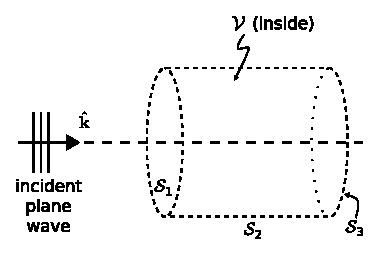
\includegraphics[width=0.8\columnwidth]{modules/m0122_fPTE.eps} 
% https://commons.wikimedia.org/wiki/File:Uniform_plane_wave_incident_cylindrical_surface.svg
}}{A horizontal cylinder with inside region labeled capital V. The leftmost circular surface is capital S subscript 1, the cylindrical surface capital S subscript 2 and the rightmost circular surface is capital S subscript 3. Incident plane wave, represented by 3 vertical lines, is boldface small k hat points toward capital S subscript 1.}
\end{center}
\centerline{\scriptsize 
\copyright~\hyperref[m0122_fPTE_Credit]{C.\ Wang} 
\href{https://creativecommons.org/licenses/by-sa/4.0/}{CC BY-SA 4.0} 
} 
\caption{
\label{m0122_fPTE}
A uniform plane wave incident on a region bounded by the cylindrical surface $\mathcal{S}$.
}
\end{figure}

Now let us apply Poynting's theorem:
%
\begin{equation}
P_{net,in}
= P_{\Omega}
+ \frac{\partial}{\partial t} W_e
+ \frac{\partial}{\partial t} W_m
\end{equation}
%
Since the region is lossless, $P_{\Omega}=0$.
Presuming no other electric or magnetic fields, $W_e$ and $W_m$ must also be zero.
Consequently, $P_{net,in}=0$. 
However, this does \emph{not} mean that there is no power flowing into $\mathcal{V}$.  
Instead, $P_{net,in}=0$ merely indicates that the \emph{net} power flowing into $\mathcal{V}$ is zero. 
Thus, we might instead express the result for the present scenario as follows:
%
\begin{equation}
P_{net,in} = P_{in}-P_{out} = 0
\label{m0122_ePB}
\end{equation} 
%
where $P_{in}$ and $P_{out}$ indicate power flow explicitly into and explicitly out of $\mathcal{V}$ as separate quantities.

Proceeding, let's ignore what we know about power flow in plane waves, and instead see where Poynting's theorem takes us.  Here,
%
\begin{equation}
P_{net,in} \triangleq -\oint_{\mathcal{S}} \left( {\bf E} \times {\bf H} \right) \cdot d{\bf s} = 0
\end{equation} 
%
The surface $\mathcal{S}$ consists of three sides: The two flat ends, and the curved surface that connects them.  Let us refer to these sides as $\mathcal{S}_1$, $\mathcal{S}_2$, and $\mathcal{S}_3$, from left to right as shown in Figure~\ref{m0122_fPTE}.  Then,
%
\begin{flalign}
-&\int_{\mathcal{S}_1} \left( {\bf E} \times {\bf H} \right) \cdot d{\bf s} \\ \nonumber
-&\int_{\mathcal{S}_2} \left( {\bf E} \times {\bf H} \right) \cdot d{\bf s} \\ \nonumber
-&\int_{\mathcal{S}_3} \left( {\bf E} \times {\bf H} \right) \cdot d{\bf s} = 0
\end{flalign}
%
On the curved surface $\mathcal{S}_2$, $d{\bf s}$ is everywhere perpendicular to ${\bf E} \times {\bf H}$ (i.e., perpendicular to $\hat{\bf k}$).  
Therefore, the second integral is equal to zero.
On the left end $\mathcal{S}_1$, the outward-facing differential surface element $d{\bf s} = -\hat{\bf k}ds$.
On the right end $\mathcal{S}_3$, $d{\bf s} = +\hat{\bf k}ds$.
We are left with:
%
\begin{flalign}
 &\int_{\mathcal{S}_1} \left( {\bf E} \times {\bf H} \right) \cdot \hat{\bf k}ds \\ \nonumber
-&\int_{\mathcal{S}_3} \left( {\bf E} \times {\bf H} \right) \cdot \hat{\bf k}ds = 0
\end{flalign}
%
Compare this to Equation~\ref{m0122_ePB}.
Since $\hat{\bf k}$ is, by definition, the direction in which ${\bf E} \times {\bf H}$ points, the first integral must be $P_{in}$ and the second integral must be $P_{out}$.
Thus,
%
\begin{equation}
P_{in} = \int_{\mathcal{S}_1} \left( {\bf E} \times {\bf H} \right) \cdot \hat{\bf k}ds 
\end{equation}
%
and it follows that the magnitude and direction of ${\bf E}\times{\bf H}$, which we recognize as the Poynting vector, are spatial power density and direction of power flow, respectively.  

The Poynting vector is named after English physicist J.H. Poynting, one of the co-discoverers of the concept.  The fact that this vector points in the direction of power flow, and is therefore also a ``pointing vector,'' is simply a remarkable coincidence.

%%%%%%%%%%%%%%%%%%%%%

{\bf Additional Reading:}
\begin{itemize}
\item ``\href{https://en.wikipedia.org/wiki/Poynting_vector}{Poynting vector}'' on Wikipedia.
\end{itemize}

\index{Poynting vector|)}
